\section{Introducción}
En este capítulo se describe la implementación de los componentes del framework
y se detallan sus interfaces de programación.
Se detalla la implementación de un controlador de acción y el
proceso de ejecución de los mismos. A su vez, se detalla la implementación de
los tópicos.

La implementación se realizó de acuerdo a los aspectos de diseño
expuestos en el capítulo~\ref{cap:diseno_framework}.

\section{Detalles de Implementación de \nombreFramework \ Framework}
\nombreFramework \ Framework es de un tipo intermedio entre caja negra
y caja blanca. Para utilizar la mayor parte de las funcionalidades ofrecidas, el
usuario sólo debe conocer las interfaces que expone el framework para conectar
los componentes. Sin embargo, para determinados casos de uso (por ejemplo para
añadir políticas de disparo de transiciones) se requiere de la extensión de
clases del framework.
(ver sección~\ref{sec:tipos_framework}).
El usuario tiene la responsabilidad de definir los siguientes componentes,
previamente expuestos en el capítulo~\ref{cap:diseno_framework}:
\begin{itemize} 
  \item Controladores de acciones.
  \item Tópicos.
  \item Modelo de la lógica del sistema en RdP.
\end{itemize}

Por su lado, el framework se encarga de:
\begin{itemize} 
  \item Proveer interfaces para interconectar los componentes definidos por el
  usuario.
  \item Controlar el flujo de ejecución del programa.
\end{itemize}

\section{Implementación de un Controlador De Acción}
\label{sec:implementacion_controlador_accion}
La implementación de un controlador de acción queda definida por dos elementos:
\begin{labeling}{description}
  \item [Acción a realizar: ] Método con una anotación de Java
  identificando el tipo de controlador de acción. 
  Dicha anotacion puede ser de dos tipos:
  \begin{itemize}
    \item \emph{@TaskController}
    \item \emph{@HappeningController}
  \end{itemize}
  \item [Ejecutante de la Acción: ] Es la instancia del objeto que ejecuta el
  método. Este objeto pertenece a una clase que contiene la declaración
  del método.
\end{labeling}

\section{Componentes del Framework}
\label{sec:componentes_baboon}
En la Figura~\ref{fig:diagrama_componentes} se pueden observar los
módulos que componen el framework implementado:
\begin{itemize}
  \item \textbf{BaboonConfig: } Este componente se encarga de manejar la
  suscripción de controladores de acciones a los tópicos (eventos de acción).
  Para ello provee interfaces para:
	  \begin{itemize}
	    \item Recibir el archivo de tópicos definido por el usuario
	    \emph{(addTopics)}.
	    \item Suscribir los controladores de acciones a tópicos específicos
	    \emph{(subscribeToTopic, createNewComplexTask, appendTaskToComplexTask)}.
	    \item Consultar las suscripciones existentes
	    \emph{(getTaskControllerSubscription,
	    getHappeningControllerSubscripton)}.
	  \end{itemize}
	  
  \item \textbf{PetriCore: } Este componente es un wrapper sobre el monitor de
  Redes de Petri descripto en el
  Capítulo~\ref{cap:petri_monitor}, y provee las interfaces del
  monitor al resto del framework.
  
  \item \textbf{BaboonApplication: } Es una interfaz Java que define dos
  métodos. Esta interfaz debe ser implementada por una clase de usuario, que
  será utilizada para inicializar el sistema. Los métodos son:
      \begin{itemize}
        \item \textbf{\emph{declare(): }} En este método el usuario debe:
        	\begin{enumerate}
        	  \item Proveer un archivo JSON con la definición de los tópicos.
        	  \item Proveer un archivo PNML con la definición del modelo de RdP.
        	  \item Declarar e inicializar los objetos del sistema. Estos objetos
        	  (desarrollados por el usuario) contienen la implementación
        	  de los controladores de acción.
        	\end{enumerate}
        \item \textbf{\emph{subscribe(): }} En este método el usuario define todas
        las suscripciones de controladores de acción a tópicos.
       \end{itemize}
   
  \item \textbf{DummyThread: } Objeto que implementa la interfaz Callable y, en
  consecuencia, es ejecutable por un hilo. Encapsula el controlador de acción
  con los eventos lógicos necesarios para su sincronización. Se lo denomina
  ``dummy'' (tonto) porque no posee información propia, simplemente envía los
  eventos de sincronización de acuerdo a los contenidos del tópico y ejecuta
  las acciones embebidas en el TaskController.
  
  \item \textbf{DummiesExecutor: } Pool de hilos encargado de ejecutar los
  objetos DummyThread.
  
  \item \textbf{HappeningControllerJoinpointReporter: } Aspect donde se
  definen los puntos de unión del sistema y los advices que se aplican en
  dichos puntos.
  Es observable por aquellos objetos que implementen la interfaz
  JoinPointObserver.
  Los puntos de union se alcanzan:
  	\begin{itemize}
  	  \item  En el momento previo a iniciar la ejecución de un
  	  método anotado con \emph{@HappeningController}.
  	  \item En el momento posterior a finalizar la ejecución de un
  	  método anotado con \emph{@HappeningController}.
  	\end{itemize}
  Durante la ejecución del advice se realiza una actualización sobre los
  observadores suscriptos al objeto, brindando el estado del joinpoint
  alcanzado. El estado del joinpoint permite identificar a un
  HappeningController en particular a partir de la instancia de objeto que hizo
  el llamado a ejecución, y de la firma del método que se llamó a ejecutar (ver
  Sección~\ref{sec:implementacion_controlador_accion}).
  
  \item \textbf{HappeningControllerSyncronizer: } Objeto que implementa la
  interfaz JoinPointObserver. Se suscribe como observador del objeto
  HappeningControllerJoinpoint. Cuando se alcanza un joinpoint, intercambia con
  el monitor los eventos lógicos necesarios para la sincronización del
  HappeningController. Obtiene los eventos lógicos utilizando las
  interfaces de BaboonConfig para consultar las suscripciones a tópicos.
  
  \item \textbf{Main: } Componente que contiene el método principal del
  programa. Al existir inversión de control, el método main forma parte del
  framework y no debe ser implementado por el usuario.
\end{itemize}

\begin{figure}[H]
	%\vspace*{-4cm} % Estaba pisando parte del texto por esto
	\hspace{-1,60cm}
	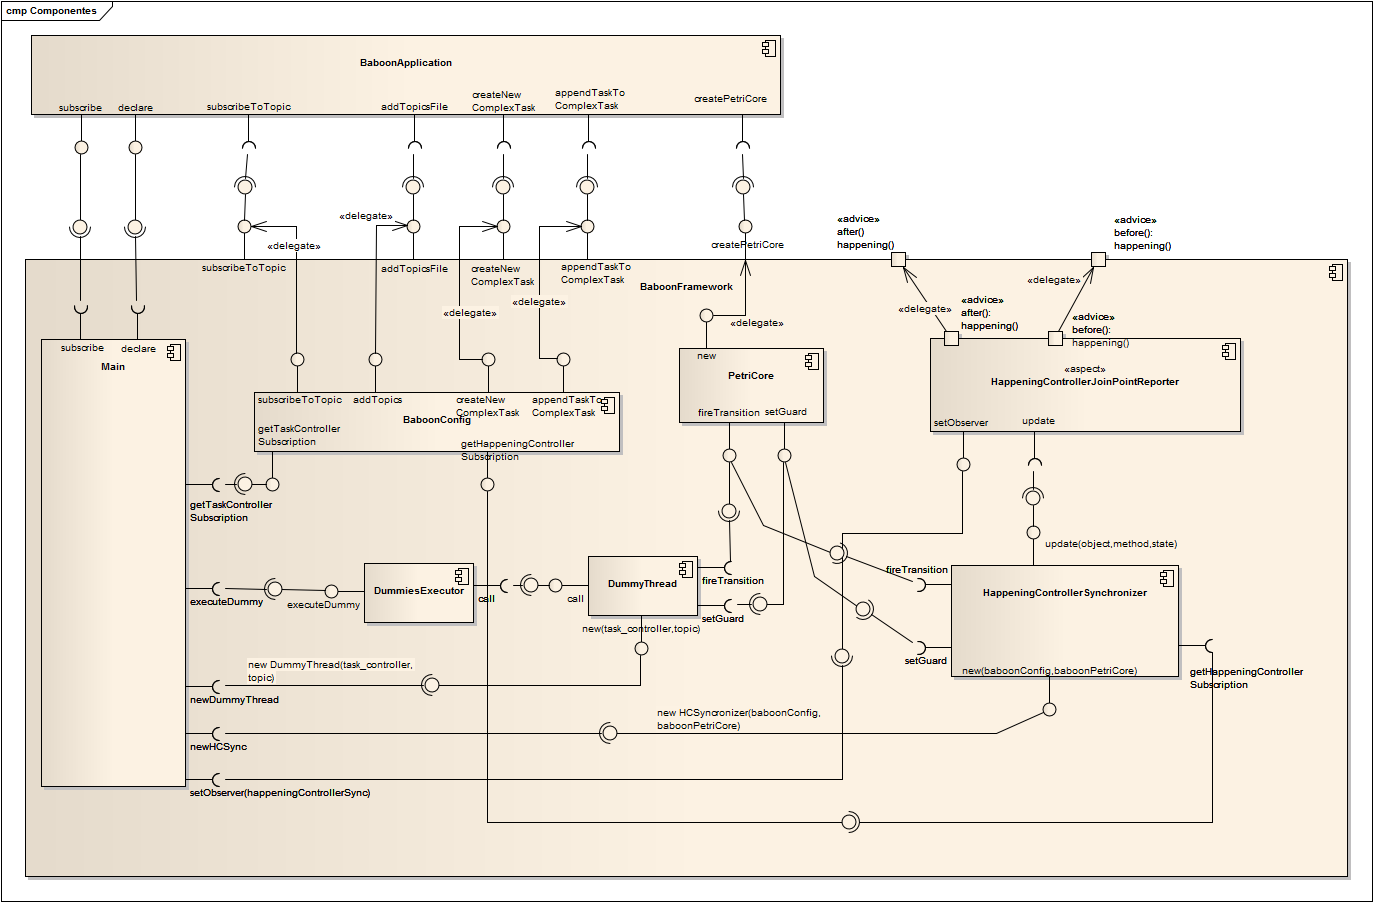
\includegraphics[width=150mm]{diagrama_componentes}
	\caption{Diagrama de Componentes de la implementación de \nombreFramework
	Framework}
	\label{fig:diagrama_componentes}
\end{figure}


\section{Ejecución de \nombreFramework \ Framework}

\begin{itemize}
  \item \textbf{Main: } La ejecución de este método consta de
  los siguientes pasos (ver
  Figura~\ref{fig:diagrama_secuencia_implementacion_ejecucion_main}):
  	\begin{enumerate}
  	  \item Obtiene la clase de usuario que implementa la interfaz
  	  BaboonApplication (utilizando Reflection) e instancia un nuevo objeto de
  	  dicha clase.
  	  \item Ejecuta los métodos declare() y subscribe() (en ese orden) del
  	  objeto mencionado en el punto anterior.
  	  \item Crea el Objeto HappeningControllerSyncronizer y lo suscribe
  	  como observer de HappeningControllerJoinPoint.
  	  \item Utiliza las interfaces de BaboonConfig para obtener las
  	  suscripciones a tópicos de los Task Controllers.
  	  \item Encapsula los TaskControllers en DummyThreads y los envía al objeto
  	  DummiesExecutor para su ejecución.
  	\end{enumerate}
  	
 \begin{figure}[H]
	\hspace{-2,90cm}
	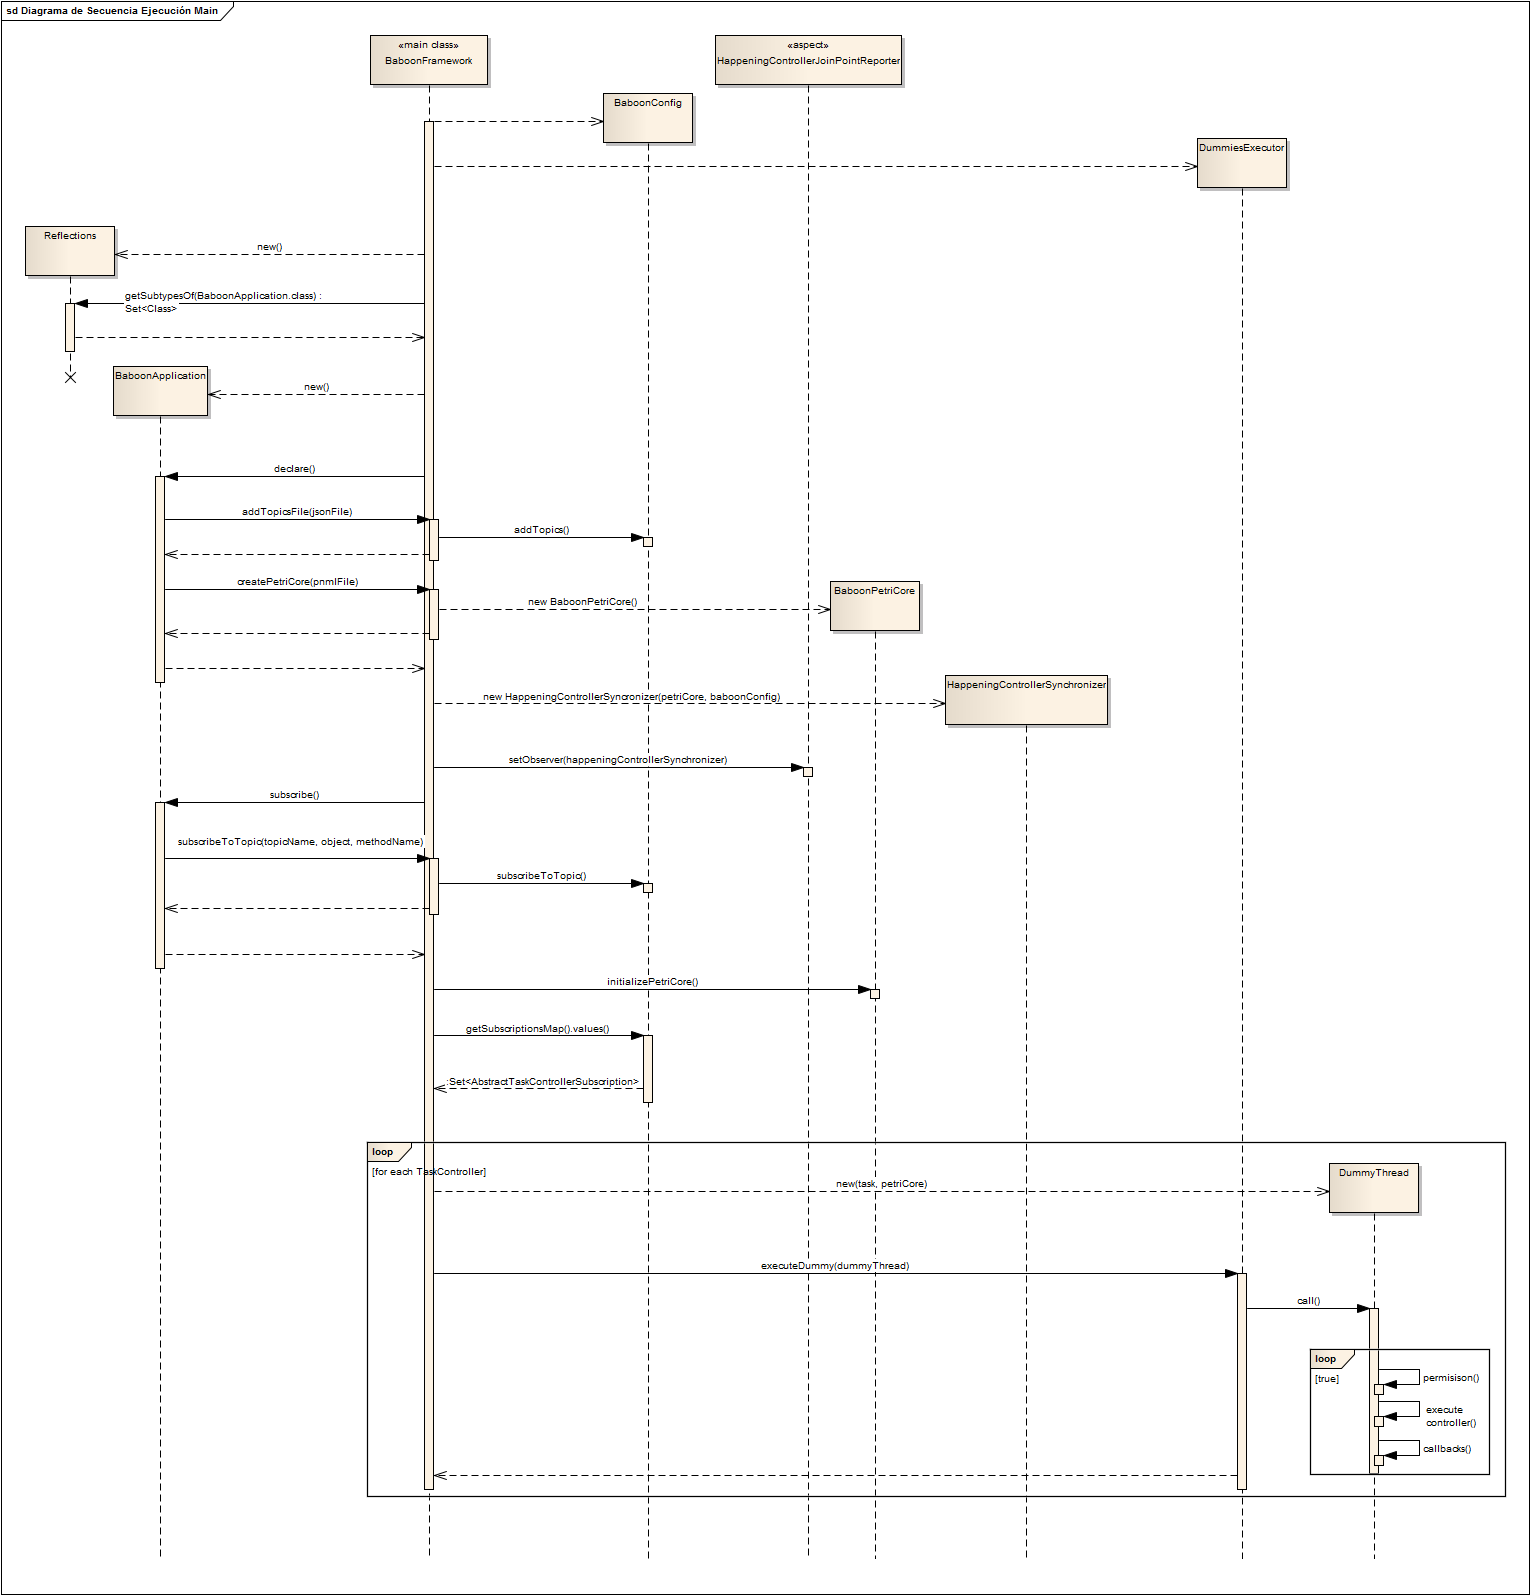
\includegraphics[width=180mm]{secuencia_implementacion_ejecucion_main}
	\caption{Diagrama de Secuencia de la Implementación del Método Principal}
	\label{fig:diagrama_secuencia_implementacion_ejecucion_main}
\end{figure}


  \item \textbf{TaskController: } La ejecución del TaskController implementada
  consta de los siguientes pasos (ver
  Figura~\ref{fig:diagrama_secuencia_implementacion_ejecucion_task_controller}):
  	\begin{enumerate}
  	  \item El pool de hilos DummiesExecutor llama a ejecutar el método
  	  \emph{call()} del DummyThread.
  	  \item El método \emph{call()} del DummyThread inicia un bucle infinito
  	  \item Utilizando el tópico de la suscripción se obtiene la transición que
  	  conforma el permiso de ejecución.
  	  \item El DummyThread realiza un disparo perenne de la transición de permiso
  	  de ejecución.
  	  \item Cuando el hilo que ejecuta al DummyThread es liberado por el
  	  monitor, llama a ejecutar el método del TaskController.
  	  \item El código del TaskController emite un evento físico de salida
  	  (Evento Task).
  	  \item Una vez finalizada la ejecución, se obtienen los nombres de las guardas asociadas al
  	  controlador a través del tópico de la suscripción.
  	  \item Se ejecutan los métodos GuardProvider que corresponden a las guardas
  	  asociadas. 
  	  \item El objeto DummyThread setea en el monitor de Petri, para cada guarda asociada, el valor
  	  correspondiente que retornan los métodos GuardProvider.
  	  \item Se obtienen del tópico los nombres de las transiciones de aviso de
  	  finalización de ejecución.
  	  \item El objeto DummyThread realiza disparos no perennes de las
  	  transiciones de aviso de finalización.
  	  \item Se repite el bucle infinito del método \emph{call()} del DummyThread.
  	\end{enumerate}
  	
\begin{figure}[H]
	\hspace{-2,90cm}
	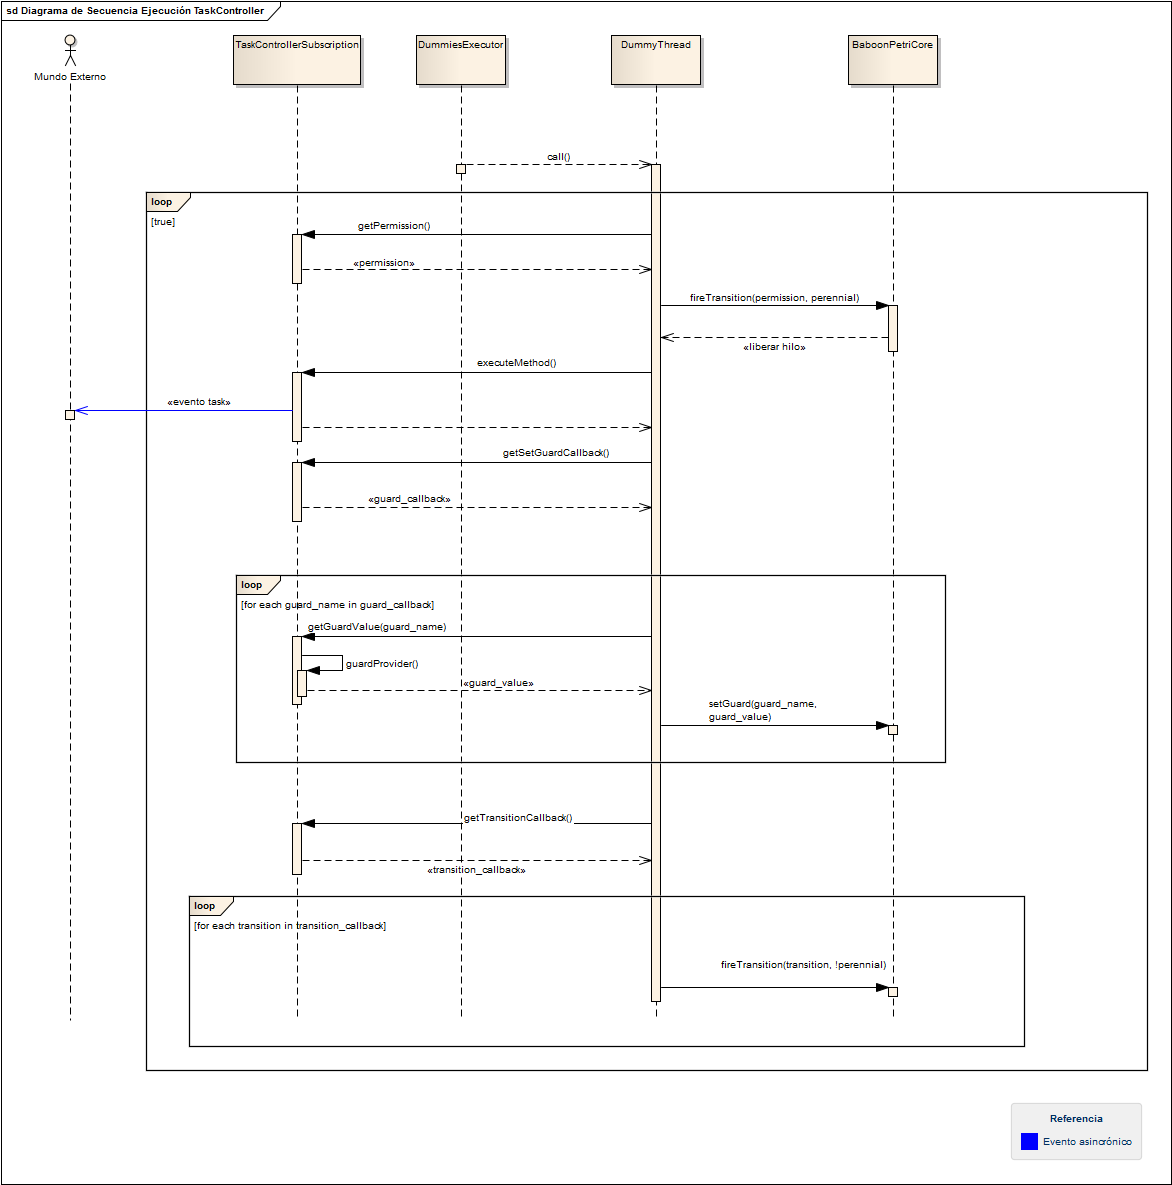
\includegraphics[width=180mm]{secuencia_implementacion_ejecucion_task_controller}
	\caption{Diagrama de Secuencia de la Ejecución Implementada de un
	TaskController}
	\label{fig:diagrama_secuencia_implementacion_ejecucion_task_controller}
\end{figure}

  \item \textbf{HappeningController: } La ejecución implementada de un
  HappeningController es de la siguiente forma (ver
  Figura~\ref{fig:diagrama_secuencia_implementacion_ejecucion_happening_controller}):
  	\begin{enumerate}
  	  \item El código de usuario recibe un evento asincrónico del Mundo Exterior
  	  (Evento Happening).
  	  \item El código de usuario realiza en un hilo el llamado a ejecución del
  	  HappeningController encargado de manejar el Evento Happening.
  	  \item En este punto de la ejecución se alcanza un joinpoint, por lo tanto
  	  antes de ejecutar el HappeningController se ejecuta el advice
  	  \emph{before()} del objeto HappeningControllerJoinPoint.
  	  \item El advice \emph{before()} realiza un update del estado del joinpoint
  	  al objeto HappeningControllerSincronizer.
  	  Dicho estado se compone del nombre del método anotado con
  	  \emph{@HappeningController} que se llamó a ejecución, de la instancia del
  	  objeto que invocó dicho método y de un enum que indica que el joinpoint es
  	  previo a la ejecución del controlador.
  	  \item El HappeningControllerSincronizer obtiene de BaboonConfig la
  	  suscripción al tópico del HappeningController, a partir de los datos
  	  obtenidos del estado del joinpoint.
  	  \item Utilizando el tópico de la suscripción se obtiene la transición que
  	  conforma el permiso de ejecución.
  	  \item El HappeningControllerSincronizer realiza un disparo perenne de la
  	  transición de permiso de ejecución.
  	  \item  Cuando el hilo de ejecución es liberado por el monitor, se ejecuta
  	  el código del HappeningController, donde se maneja el evento recibido.
  	  \item Al finalizar la ejecución del HappeningController se alcanza un
  	  joinpoint, y se ejecuta el advice \emph{after()} del objeto
  	  HappeningControllerJoinPoint.
  	  \item El advice \emph{after()} realiza un update del estado del joinpoint
  	  al objeto HappeningControllerSincronizer. Este estado es similar al
  	  descripto en el advice \emph{before()}, con la diferencia de que en este
  	  caso el enum indica que el joinpoint es posterior a la ejecución del
  	  controlador.
  	  \item El HappeningControllerSincronizer obtiene de BaboonConfig la
  	  suscripción al tópico del HappeningController, a partir de los datos
  	  obtenidos del estado del joinpoint.
  	  \item Se obtienen los nombres de las guardas asociadas al controlador a
  	  través del tópico de la suscripción.
  	  \item Se ejecutan los métodos GuardProvider que corresponden a las guardas
  	  asociadas.
  	  \item El objeto HappeningControllerSincronizer setea en el monitor de
  	  Petri, para cada guarda asociada, el valor correspondiente que retornan los métodos GuardProvider.
  	  \item Se obtienen del tópico los nombres de las transiciones de aviso de
  	  finalización de ejecución.
  	  \item El objeto HappeningControllerSincronizer realiza disparos no perennes
  	  de las transiciones de aviso de finalización.
  	\end{enumerate}
  	
  	\begin{framed}
	\textbf{Nota:} Los advices de AspectJ implementados se ``tejen'' al código de
	usuario en tiempo de compilación (ver Sección~\ref{sec:aop_terminologia}).
	Dichos advices son ejecutados por el mismo hilo que el HappeningController que
	produce el joinpoint. De esta forma, el hilo que realiza los disparos de
	transición desde el objeto HappeningControllerSincronizer es el mismo que
	ejecuta el controlador de acción, permitiendo su sincronización.
	\end{framed}



\begin{figure}[H]
	\hspace{-2,90cm}
	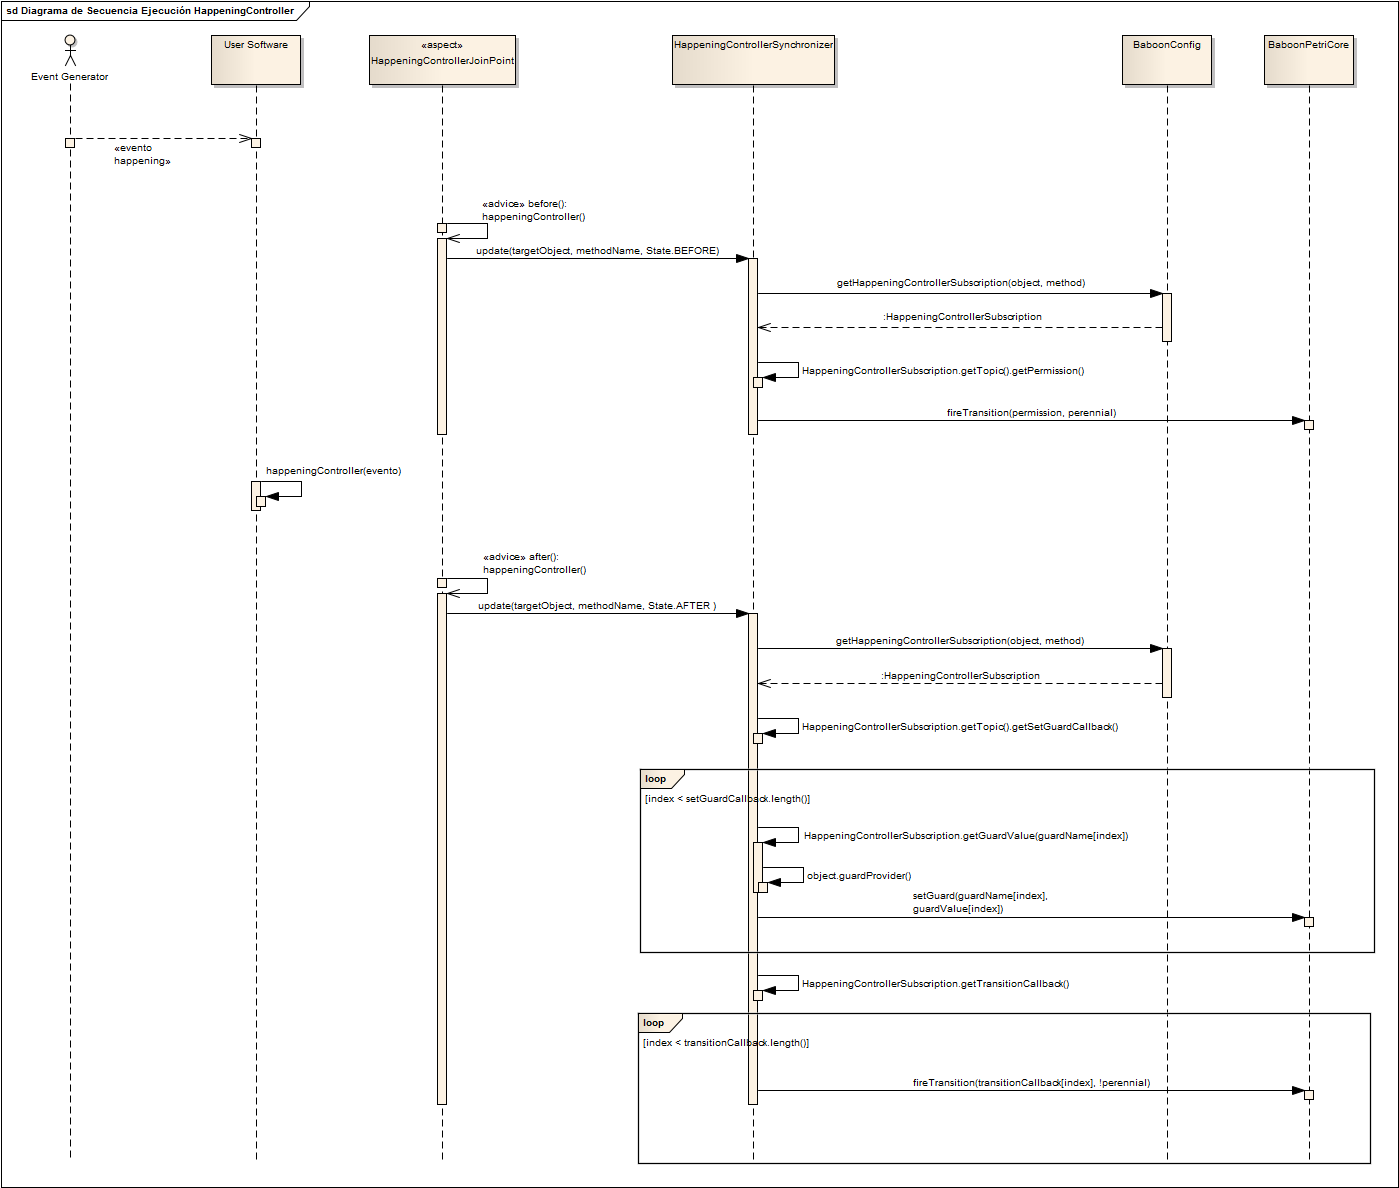
\includegraphics[width=180mm]{secuencia_implementacion_ejecucion_happening_controller}
	\caption{Diagrama de Secuencia de la Ejecución Implementada de un
	HappeningController}
	\label{fig:diagrama_secuencia_implementacion_ejecucion_happening_controller}
\end{figure}

\end{itemize}

\section{Implementación de Tópicos}
Los tópicos, cuyo concepto se explica en la sección \ref{sec:diseno_topicos}, son definidos
por el usuario en un archivo de formato JSON, de la forma que se presenta a
continuación:
\begin{minted}{json}
[

  {
    "name":"custom_name_1",
    "permission":["my_p", "my_p2", "my_p3"],
    "setGuardCallback": [["g1","g3"],["g1","g2"],["g2","g3"]]
    "fireCallback":["fc_1","fc_2"]
  },
  
  {
    "name":"test",
    "permission":["my_permission", "my_permission2", "perm3", "p4"],
    "setGuardCallback": [["g1","guard2","g3"],["guardaCuatro"],[],["g5","g_6"]] 
  },
  
  {
    "name":"test",
    "permission":["my_transition"],
  },
  
  {
    "name":"topicN",
    "permission":["transition0"],
    "fireCallback":["t1","t2","tx"]
  }
]
\end{minted}

El path a este archivo es incluido en el software de usuario al momento de
inicializar \nombreFramework framework. Un parser interno del framework se
encarga de procesar este archivo JSON y asociar el tópico a los eventos
lógicos.

Una vez configurado y cargado en el sistema el archivo de tópicos, el usuario
puede usar el valor de ``name'' del tópico como identificador para suscribir
los controladores de acciones.
